In the following we will consider two DAGs, each with some particular nodes called head. The set of heads is the smallest set so that every node in the considered DAG is an ancestor of one of the head. One of the DAG will be refered to as Client or $Bob$ and the other one as Server or $Alice$. $\mathrm{Ancestor}(Alice)$ and $\mathrm{Ancestor}(Bob)$ are the considered DAGs and the aim of the algorithm is to be able to compute $\mathrm{Ancestor}(Alice) \setminus \mathrm{Ancestor}(Bob) = \{ x\ ,\ x \in \mathrm{Ancestor}(Alice) \wedge x \notin \mathrm{Ancestor}(Bob)\}$. The complexity of the algorithm will be expressed in terms of $n = \#(\mathrm{Ancestor}(Alice) \setminus \mathrm{Ancestor}(Bob))$. In terms of application, the client and the server are two entities that are physically distinct, therefore it was important during the design of the algorithm to keep in mind and to be aware that :
\begin{enumerate}
 \item The quantity of information exchanged between the two processes shall be the smaller possible
 \item We want to minimise the complexity on both processes
 \item There can be no no pre-assumptions on the shape of the graph, because the shape of the global DAG (with multiple head) is evolving in time and is not known at the beginning.
 \item There is no high authority that has a memory of every thing.
\end{enumerate}
\paragraph{} The section~\ref{sec:prelim} underlined that we were not able to find a way to compute easily the set of BCA, moreover if the server has to send the difference $\mathrm{Ancestor}(Alice) \setminus \mathrm{Ancestor}(Bob)$ then at some point we will have to go all over this difference, therefore we decided that the server could cross the part of its history corresponding to the difference.
% However the server does not know what nodes are already in the history of the client. Hence the client need to send to the server its history so that the server knows when the exploration of its past shal stop. Sending all of the client's history can requiere a huge exchange of data, moreover in applications we are interested in (git) the difference we are trying to compute is usually small compared to the size of the all history. the client shall therefore only send the latest event in its history (a fixed number) so that in most case the server manages to make the link between the two histories. However 
% in some cases the server will not be able to find any of the client's latest node in its history, in such cases the server will have to go throw all of its history (because the link can be anywhere) to understand that it has nothing in common with this set of latest nodes. We do not want the server to go throw all of its history as we have no bound on the size of this history. Thus the client need to tell the server that at some point of its exploration the server need to stop because there is no point in continuing the exploration. We introduce the Border of a set of nodes $A$ as defined such that for every nodes in $A$ each of its predecessor are either in $A$ or in the border of $A$. To sum up, the client divides its history in packages that will be called "window" and to each window we associate a "border" (see \ref{fig:twoproc}). Now if the client send a window and the union of all the borders to the server, this one will, at some point, find one of the two while exploring its history bottom-up and 
% therefore will not have to go across all of its history.
\begin{definition}
 Given a DAG $\mathcal{D}$ and a partition of a the nodes of $\mathcal{D}$, we call a set of equivalent nodes for this partition a "slice of $\mathcal{D}$"
\end{definition}
\begin{definition}
 Given a DAG $\mathcal{D}$ and a slice $\mathcal{S}$ we call the border of $\mathcal{S}$ (noted $\overline{\mathcal S}$) the smallest set such that $\forall x \in \mathcal{D},\ \forall y\in \mathrm{predecessor}(x)\  y\in \mathcal{S} \vee y \in \overline{\mathcal S}$.
\end{definition}
\paragraph{Idea of the algorithm} We assume that a partition of its DAG of ancestors is known by the client as well as well as a border for every slice of the partition.
\begin{enumerate}
 \item The client sends the list of its head, one of its slice and the union of all the border to the Server
 \item The server goes up in its history and stop whenever it crosses a node in the slice are in the border.
 \item The server computes the DAG $D$ of the successors of every nodes it found in slice.
 \item The server computes a list of "nodes of interest" from which it shall starts again the exploration (those "nodes of interest" are the last successors of the nodes found in the border that are not in $D$)
 \item The server sends back $D$ and the list of "nodes of interest"
 \item The client starts again with anoter slice and instead of the list of its head it sends the list of "nodes of interest" it received from the server, except if there is no "node of interest" in which case the algorithm stop.
\end{enumerate}
\paragraph{} This algorithm as the property that the server have absolutely no memory. The figure~\ref{fig:twoproc} shows a partition of two dags in slices.

\begin{figure}[H]
\centering
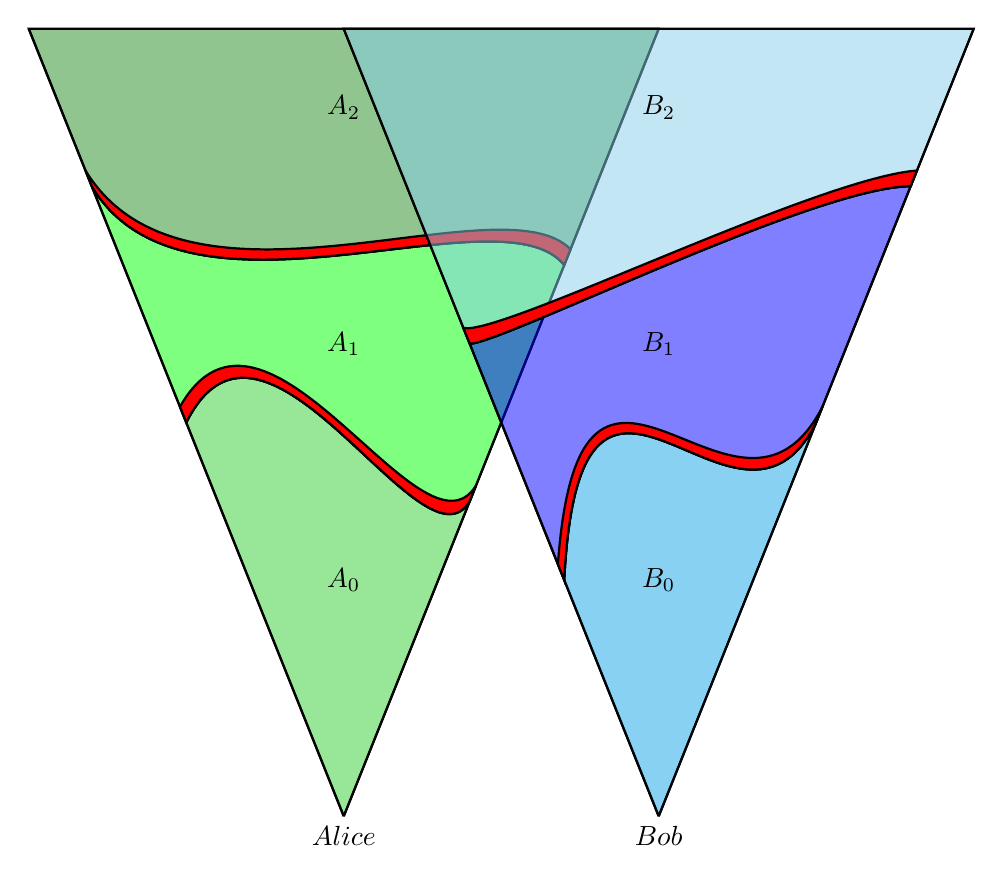
\begin{tikzpicture}
\begin{scope}
\coordinate[label=below:$Alice$] (A) at (0,0) ;
\coordinate (B) at (4,10);
\coordinate (C) at (-4,10);
\draw [thick] (A) -- (B) coordinate[pos = 0.4] (B1) {} coordinate [pos = 0.42] (B1b) {} coordinate[pos = 0.7] (B2) {} coordinate[pos = 0.72] (B2b) {};
\draw [thick] (B) -- (C) coordinate[pos = 0.5] (midBC) {};
\draw [thick] (A) -- (C) coordinate[pos = 0.5] (C1) {} coordinate [pos = 0.52] (C1b) {} coordinate[pos = 0.8] (C2) {} coordinate[pos = 0.82] (C2b) {};
\draw [thick, fill = LimeGreen,fill opacity = 0.5] (A) -- (B1) .. controls (1,3) and (-1,7) .. (C1) -- (A);
\draw [thick, fill = green,fill opacity = 0.5] (B1) .. controls (1,3) and (-1,7) .. (C1) -- (C2) .. controls (-2,6) and (2,8) .. (B2) -- (B1);
\draw [thick, fill = ForestGreen, fill opacity = 0.5] (C2) .. controls (-2,6) and (2,8) .. (B2) -- (B) -- (C) -- (C2);
\draw [thick, fill = red, fill opacity = 1] (B1b) .. controls (1,3.1) and (-1,7.1) .. (C1b) -- (C1) .. controls (-1,7) and (1,3) .. (B1) -- (B1b);
\draw [thick, fill = red, fill opacity = 1] (C2) .. controls (-2,6) and (2,8) .. (B2) -- (B2b) .. controls (2,8.1) and (-2,6.1) .. (C2b) -- (C2);
\draw [draw = none] (A) -- (midBC) node[pos = 0.3] {$A_0$} node[pos = 0.6] {$A_1$} node[pos = 0.9] {$A_2$};

\end{scope}
\begin{scope}[shift={(4cm,0cm)}]
\coordinate[label=below:$Bob$] (D) at (0,0);
\coordinate (E) at (4,10);
\coordinate (F) at (-4,10);
\draw [thick] (D) -- (E) coordinate[pos = 0.5] (E1) {} coordinate [pos = 0.52] (E1b) {} coordinate[pos = 0.8] (E2) {} coordinate[pos = 0.82] (E2b) {};
\draw [thick] (E) -- (F) coordinate[pos = 0.5] (midEF) {};
\draw [thick] (D) -- (F) coordinate[pos = 0.3] (F1) {} coordinate [pos = 0.32] (F1b) {} coordinate[pos = 0.6] (F2) {} coordinate[pos = 0.62] (F2b) {};
\draw [thick, fill = Cerulean,fill opacity = 0.5] (D) -- (E1) .. controls (1,3) and (-1,7) .. (F1) -- (D);
\draw [thick, fill = blue,fill opacity = 0.5] (E1) .. controls (1,3) and (-1,7) .. (F1) -- (F2) .. controls (-2,6) and (2,8) .. (E2) -- (E1);
\draw [thick, fill = SkyBlue, fill opacity = 0.5] (F2) .. controls (-2,6) and (2,8) .. (E2) -- (E) -- (F) -- (F2);
\draw [thick, fill = red, fill opacity = 1] (E1b) .. controls (1,3.1) and (-1,7.1) .. (F1b) -- (F1) .. controls (-1,7) and (1,3) .. (E1) -- (E1b);
\draw [thick, fill = red, fill opacity = 1] (F2) .. controls (-2,6) and (2,8) .. (E2) -- (E2b) .. controls (2,8.1) and (-2,6.1) .. (F2b) -- (F2);
\draw [draw = none] (D) -- (midEF) node[pos = 0.3] {$B_0$} node[pos = 0.6] {$B_1$} node[pos = 0.9] {$B_2$};
\end{scope}
\end{tikzpicture}
\caption{Two processes sharing a part of their history and their decomposition in Slices and Borders} \label{fig:twoproc}
\end{figure}
The figure~\ref{fig:twoproc} underlines the fact that it is interesting to have a interesting partition of the node, in the sense that :
\begin{enumerate}
 \item We want the borders to be small so that we do not have to send a lot of information
 \item We want to do the least sending/receiving data to/from the server possible
 \item We want those slices/border to be easy to compute, in the sense that we do not want to cross all of the history of the client each time we want to merge
 \item We want the slices to be all of the same size
\end{enumerate}
Let us assume we decided that the slices should be of size $n$ and that a process already knows a partition $\mathcal{P} = \{A_0,\cdots,A_m\}$ in slices of its ancestors and the paired borders. This process needs to add some nodes $S$ in its history. We start by filling the set in the partition with a size smaller that $n$, by adding the element from $S$ in an order verifying the order of the DAG. Therefore if $S$ contains two nodes $a$ and $b$, $a$ being a predecessor of $b$ then $a$ will be added prior than $b$. Once every partition is of size $n$ we add a new slice to $\mathcal P$. While adding a node in one of the slices we add it in the border if one of its parents is not in the slice. The order in which we add the elements ensures us that the border will be the small (regarding the number of element in the slice). Hence we can build a new partition and the corresponding borders quite easily from the previous one. Finally in order to ensure that there is not a lot of exchanges between the client and the 
server, the client send its slices from the newest to the oldest one. For example in figure~\ref{fig:twoproc} Bob will be sending the slices in the order $B_0$ then $B_1$ then $B_2$.

\paragraph{} As this algorithm is designed for multi processes, we wrote functions that can be used on the client side and on the server sides. Such functions are placed in a functor with the following signature :
\begin{lstlisting}
 module Make :
  functor (B : Graph.Sig.I) ->
    functor (D : DataSig with type t = B.V.t) ->
sig
  type v
  (** type t is the main type, it contains the ancestor dag of the set
      of nodes it represents as well as the datastructure *)
  type t
  val empty_state : unit -> t
  (** [next_ring il ia bf bd] is the function that computes the list
      of the next interesting nodes and the ring of nodes where [il]
      is the list of previous interesting nodes and [ia] is the
      ancestors list of the interesting nodes and [bf] is the current
      bloomfilter and [bd] the current border*)
  val next_ring : B.V.t list -> B.t list -> D.u -> D.u -> (B.t * (B.V.t list))
  (** [increase_high s old_hd_l new_hd] is the function that computes
      the state of new_hd where [s] is the state corresponding to the
      union of new_hd's fathers and [old_hd_l] is the list of new_hd's
      fathers and [new_hd] is new_hd *)
  val increase_high :  t ->  B.V.t list -> B.V.t -> t
  (** [increase_width s f hd] is the function that computes the state
      of the union of nodes where [s] was the state of the first nodes and
      [f] is the callback function and [hd] is the next node to be added
      to the state *)
  val increase_width : t -> ( D.u -> D.u -> B.V.t list -> (B.V.t list * B.t)) -> B.V.t -> t
end
\end{lstlisting}
\paragraph{Arguments} B is the DAGs signature and D is a datastructure module that enables merge and membership queries (for complete signature see section~\ref{sec:datasig}).
\paragraph{Invariants} In order to explain the way these functions work, we detailed some invariants on those functions.
\begin{enumerate}
 \item \label{itm:first} If $\texttt{il}$ is a list of nodes in the history of $A$, $\texttt{ia}$ is the list of the ancestor DAGs of the elements in $\texttt{il}$, if $\texttt{bf}$ is a datastructure containing a slice of $B$ and $\texttt{bd}$ is the union of all the borders of $B$, if $\texttt{g,l} = \texttt{next\_ring il ia bf bd}$ then 
%  \begin{equation}
\begin{align*}
%  \begin{split}
 &\forall (x_0,x_1,\cdots,x_n) \in \mathrm{ancestor}(B), \\
(
&\forall i \in \{1,\cdots,n-1\},\ x_i \notin \texttt{bd}\cup\texttt{bf} \wedge (x_0 \rightarrow x_1 \rightarrow \cdots \rightarrow x_n) \wedge x_0 \in \texttt{bf} \wedge x_n \in \texttt{il}
\\ &\Rightarrow \{x_0,x_1,\cdots,x_n\} \subset \texttt{g}
% \end{split}
)\\
&\wedge \\
(
 &\exists k \in \{1,\cdots,n-1\},\ (x_k \in \texttt{g} \wedge x_{k-1} \notin \texttt{g}) \wedge (x_0 \rightarrow x_1 \rightarrow \cdots \rightarrow x_n) \wedge x_0 \in \texttt{bd} \\
 &\wedge \forall i \in \{1,\cdots,n-1\},\ x_i \notin \texttt{bd}\cup\texttt{bf} \\
 &\Rightarrow x_{i-1} \in l
)
 \end{align*}
 \item If $\texttt{s}$ is a state containing a DAG $D$ of the ancestors of a list $\texttt{old\_hd\_l}$ of nodes, then for all $\texttt{new\_hd}$, $\texttt{s'} = \texttt{increase\_high s old\_hd\_l new\_hd}$ is a state containing the DAG with head $\texttt{new\_hd}$, which fathers are $\texttt{old\_hd\_l}$ and $D$
 \item If $\texttt{s}$ is a state containing a DAG $D$, $\texttt{f}$ is a function veryfing the invariant of item \ref{itm:first} and $\texttt{t}$ is a node in $B$ then $\texttt{s'} = \texttt{increase\_width s f t}$ is a state containint the DAG $D$ as well as $t$ and all of its ancestors in $B$.
% \end{equation}
\end{enumerate}
% \begin{algorithm}[H] 
%   \SetAlgoLined
%   \caption{Finding some of the ancestors of $Alice$ not known by $Bob$}
%   \SetKwInOut{Input}{input}\SetKwInOut{Output}{output}
%   \SetKwComment{tcc}{(*}{*)}
%   \KwData{\texttt{Alice\_Heads} : some nodes in the history of $Alice$, \texttt{Ancestor} : a dag of the ancesters of $Alice$, \texttt{G\_In} : a graph of ancestors of $Alice$ not known by $Bob$, \texttt{Bf} : The Bloom filter of $Bob$, \texttt{Bd} : The Border of $Bob$}
% %   \KwData{
% %     \begin{itemize}
% %     \item \texttt{Alice\_Heads} : some nodes in the history of $Alice$
% %     \item \texttt{Ancestor} : a dag of the ancesters of $Alice$
% %     \item \texttt{G\_In} : a graph of ancestors of $Alice$ not known by $Bob$
% %     \item \texttt{Bf} : The Bloom filter of $Bob$
% %     \item \texttt{Bd} : The Border of $Bob$
% %     \end{itemize}
% %     }
%   \KwResult{\texttt{G\_Out} : a graph of ancestors of $Alice$ not known by $Bob$, \texttt{node\_to\_check} : a list of ancestors of $Alice$ that shall be revisited with the next Bloomfilters}
% %   \KwResult{
% %   \begin{itemize}
% %   \item \texttt{G\_Out} : a graph of ancestors of $Alice$ not known by $Bob$
% %   \item \texttt{node\_to\_check} : a list of ancestors of $Alice$ that shall be revisited with the next Bloomfilters
% %   \end{itemize}
% %   }
%   
% \SetAlgoLined\DontPrintSemicolon
% \SetKwFunction{explore}{\textbf{explore}}
% \SetKwFunction{belong}{\textbf{belong}}
% \SetKwFunction{addv}{\textbf{add\_vertex}}
% \SetKwFunction{adde}{\textbf{add\_edge}}
% \SetKwFunction{succ}{\textbf{successor}}
% \SetKwFunction{pred}{\textbf{predecessor}}
% \SetKwProg{myproc}{Procedure}{}{}
% \myproc{\explore{\texttt{node},\texttt{visited},\texttt{in\_bf},\texttt{in\_border}}}{
% 
%   \eIf{\belong{\texttt{node,\texttt{Bf}}}}{
%     \KwRet{(\texttt{visited} $\cup$ \texttt{node},\texttt{in\_bf} $\cup$ \texttt{node},\texttt{in\_border})}
%   }
%   {
%     \eIf{\belong{\texttt{node,\texttt{Bd}}}}{
%     \KwRet{(\texttt{visited} $\cup$ \texttt{node},\texttt{in\_bf} ,\texttt{in\_border}$\cup$ \texttt{node})}
%     }
%     {
%       \texttt{visited\_already} = \texttt{node} $\cup$ \texttt{visited}\;
%       \texttt{in\_bf\_already} = \texttt{in\_bf}\;				
%       \texttt{in\_border\_already} = \texttt{in\_border}\;
%       \For{\texttt{pere} $\in$ \pred{\texttt{Ancestor},\texttt{node}}}{
%       \If{\texttt{pere} $\notin$ \texttt{explored}}
%       {
% 	\texttt{visited\_already,in\_bf\_already,in\_border\_already} = \explore{\texttt{pere},\texttt{visited\_already},\texttt{in\_bf\_already},\texttt{in\_border\_already}}\;
%       }
%       }
%       \KwRet{(\texttt{visited\_already},\texttt{in\_bf\_already},\texttt{in\_border\_already})}\;
%     }	
%   }
% }
% 
% \SetKwFunction{bf}{\textbf{find\_in\_bf}}
% \SetKwFunction{bd}{\textbf{find\_in\_border}}
% \myproc{\bf{\texttt{node},\texttt{explored}}}{
%     \addv{\texttt{G\_In},\texttt{node}}\;
%     \texttt{already\_explored} = \texttt{explored} $\cup$ \texttt{node}\;
%     \For{\texttt{fils} $\in$ \succ{\texttt{Ancestor},\texttt{node}}}{
%       \adde{\texttt{G\_In},\texttt{node},\texttt{fils}}\;
%       \If{$\texttt{fils} \notin \texttt{already\_explored} \wedge \texttt{fils} \notin \texttt{G\_In}$}{
% 	\texttt{already\_explored} = \bf{\texttt{fils},\texttt{already\_explored}}
% 	}
%     }
%     \KwRet{already\_explored}
% }
% 
% \myproc{\bd{\texttt{node},\texttt{explored},\texttt{to\_further\_explore}}}{
%   \If{$\texttt{node} \notin \texttt{explored}$}{
%     \texttt{son\_in} = $\varnothing$\;
%     \texttt{son\_out} = $\varnothing$\;
%     \For{\texttt{fils} $\in$ \succ{\texttt{Ancestor},\texttt{node}}}{
%       \eIf{\texttt{fils} $\in$ \texttt{G\_In}}{
% 	\texttt{son\_in} = \texttt{fils} $\cup$ \texttt{son\_in}\; 
%       }{
% 	\texttt{son\_out} = \texttt{fils} $\cup$ \texttt{son\_out}\;
%       }
%     }
%     \texttt{already\_explored} = \texttt{explored}\;
%     \texttt{inter\_node} = \texttt{to\_further\_explore}\;
%     \If{\texttt{son\_in} = $\varnothing$}{
%       \texttt{inter\_node} = \texttt{node} $\cup$ \texttt{inter\_node}\;
%     }
%     \For{\texttt{fils} $\in$ \texttt{son\_out}}{
%       \If{\texttt{fils} $\notin$ \texttt{already\_explored}}{
% 	\texttt{already\_explored},\texttt{inter\_node} = \bd{\texttt{fils},\texttt{already\_explored},\texttt{inter\_node}}\;
%       }
%     }
%     \KwRet{(already\_explored,inter\_node)}\;
%   }
% }
% \end{algorithm}
  
  